\documentclass[10pt,a4paper]{article}
\usepackage[margin=2cm]{geometry}
\usepackage{amsmath,amssymb,booktabs,graphicx,caption,xcolor,float,hyperref,tikz}
\usetikzlibrary{arrows.meta,positioning,calc}
\hypersetup{colorlinks=true,linkcolor=blue!50!black,urlcolor=blue!50!black}
\captionsetup{font=small,labelfont=bf}
\title{\vspace{-1.2cm}\textbf{A larger budget, a board that forgets faster or slower}\\[2pt]
\large Simulation 2 (asynchronous activation), setup \texttt{task003-nosolution}: three variants against the gold standard}
\author{LLM-free simulator; report of 19 October 2026; runs of 15, 16 and 18 October 2026\\
\small Same sections, figures and equations as the nosolution report of 17 October (itself built like the gold standard), with the four cases side by side.}
\date{}
\begin{document}
\maketitle
\vspace{-1cm}

\paragraph{How the simulator works.} The world, \texttt{task\_003}, has three candidate allocations; A0 is the
correct one. Each of 24 agents is given one true fact and reasons as an exact Bayesian: its \emph{belief} is the
exact probability of A0, A1 and A2 given the facts it currently remembers. There are no rounds. Each agent acts
at random times, on average once per time unit: it reads $q$ posts drawn at random from the $W$ most recent posts ($W = 48$ in the gold standard)
on a shared \emph{board} (never its own), adds their facts to its memory, recomputes its belief, \emph{votes} by
probability matching (a vote drawn from its belief) and posts one remembered fact that supports its vote. Every
remembered fact is forgotten after a random lifetime (on average a fraction $\rho$ survives one time unit; reading
it again renews it). A \emph{controller} with a target, A0 (truth) or A2 (false), acts at random times at rate
$\lambda_c$ until $t = 30$: it reads $q_c$ recent agent posts and, unless the \emph{vote gate} (at least 75\% of
them from agents voting for its target) or the \emph{proof stop} (its target already proved; it cannot act in this setup) silences it, posts
the one fact from its pool that best supports its target, at most $B$ messages per episode ($B = 30$ in the gold standard). Agents continue
alone until $t = 40$. Every episode is run three times with the same random draws: without a controller
(\emph{silent}), with the controller targeting A0 and with the one targeting A2.

\paragraph{The facts at the start.} All facts are true, and no set of them proves any allocation: the agents'
evidence is a coin flip between A0 and A2, and one pool serves both targets (Table~\ref{tab:facts}).

\begin{table}[H]
\centering\small
\caption{Facts available at $t = 0$ and what each set implies, $P(\text{A0}, \text{A1}, \text{A2} \mid \text{facts})$.}
\label{tab:facts}
\begin{tabular}{lcc}
\toprule
set of facts & facts & $P(\text{A0}, \text{A1}, \text{A2})$ \\
\midrule
agents' facts, all together (24 agents, one fact each) & 15 distinct & (0.5, 0, 0.5): no proof \\
shared pool (both targets) & 12, all new to the agents & (0.37, 0.26, 0.37) \\
agents' facts + pool & 27 distinct & (0.75, 0, 0.25) \\
\bottomrule
\end{tabular}
\end{table}

\paragraph{The three variants.} Each changes one rule of the gold standard and keeps everything else
(Table~\ref{tab:cases}).

\begin{itemize}\itemsep1pt
\item \textbf{Budget.} In the gold standard the controller may post at most $B = 30$ messages before $t = 30$; from
  $\lambda_c = 2$ upward it uses almost all of them, and at $\lambda_c = 8$ it runs out near $t = 4$. With $B = 100$
  it can keep posting until $t = 30$ for $\lambda_c \lesssim 3$ and runs out near $t = 12.5$ at $\lambda_c = 8$; the
  vote gate can still silence it. This separates the rate from the total effort.
\item \textbf{Board window.} Nothing is ever deleted from the board, but every reader (agent or controller) draws
  only from the $W$ newest posts it may read. The 24 agents post about 24 times per time unit, so in the gold
  standard ($W = 48$) a post stays readable for about 2 time units unless someone posts its fact again. With
  $W = 24$ it stays about 1 time unit (a board that forgets fast); with $W = 240$ about 10 (a board that forgets
  slowly). The window also changes what the controller reads, so with $W = 240$ its vote gate sees older votes.
\end{itemize}

\begin{table}[H]
\centering\small
\caption{The four cases compared in this report. All: $q_c = 12$, $\rho \in \{1, 0.75, 0.5, 0.25\}$, $q \in \{3, 6, 12\}$,
all nine rates, gate on and off, 1{,}000 episodes per setting.}
\label{tab:cases}
\begin{tabular}{lccll}
\toprule
case & budget $B$ & window $W$ & a post stays readable & run \\
\midrule
gold standard & 30 & 48 & $\approx 2$ time units & 15--16 October (\texttt{*\_fine}) \\
$B = 100$ & 100 & 48 & $\approx 2$ & 18 October (\texttt{*\_budget100}) \\
$W = 24$ & 30 & 24 & $\approx 1$ & 18 October (\texttt{*\_window24}) \\
$W = 240$ & 30 & 240 & $\approx 10$ & 18 October (\texttt{*\_window240}) \\
\bottomrule
\end{tabular}
\end{table}

\paragraph{The runs.} In this report \emph{gold standard} means the gold-standard rules ($B = 30$, $W = 48$) applied to
\texttt{task003-nosolution}: the 16 October run behind the 17 October report, at $q_c = 12$ and
$\rho \in \{1, 0.75, 0.5, 0.25\}$. The three variants use the same grid: $q \in \{3, 6, 12\}$; rate
$\lambda_c \in \{0.5, 1, 2, 3, 4, 5, 6, 7, 8\}$; vote gate on and off; 1{,}000 episodes per setting (444 settings per
case). Unless stated otherwise: $q = 6$, $q_c = 12$, $\lambda_c = 1$, gate on. Where the budget cannot matter, the
$B = 100$ run reproduces the gold standard exactly: all silent settings, and every setting in which the
gold-standard controller never reached 30 messages (63 settings).

\paragraph{Summary.} The agents' evidence is a coin flip between A0 and A2 and nothing can be proved. \textbf{The
results of the 17 October report hold in all three variants}: either controller tips the swarm at every memory,
with full memory a faster controller gains less, and $\eta$ stays flat (Figures~\ref{fig:votes}, \ref{fig:eta},
\ref{fig:strength}). \textbf{The budget does not matter}: with 100 messages the controllers post two to three times
as many and gain at most 0.03 more; the A2 share never passes 0.81 (Figures~\ref{fig:perfact}, \ref{fig:messages}).
\textbf{The board's memory protects a little}: posts readable for 10 time units instead of 2 lower the false
controller's gain by 0.02--0.06 at $\rho \le 0.5$, posts readable for 1 time unit raise it by up to 0.03
(Figure~\ref{fig:gainA2}). Both effects are much smaller than in \texttt{task003-symmetric}.

\section{Quantities}\label{sec:quantities}

\paragraph{Votes.} With $n_{a,t}$ the number of agents whose last vote is answer $a$ at time $t$ and $N_t$ the
number of agents who have voted,
\begin{equation}\label{eq:share}
x_{a,t} = n_{a,t}/N_t .
\end{equation}
At $t = 0$ nobody has voted and we set $x_{a,0} = 0$; all agents have voted by $t \approx 5$. (The 9--14 October reports divided by 24, which counted agents who had
not yet acted as voting against the target; this inflated the apparent rise of the shares and the apparent bias of
the controller's sensing at early times.)

\paragraph{Paired susceptibility.} Following \texttt{BLACKBOARD\_OBSERVABLES\_AND\_EFFICIENCIES} (\S3), for a
controller policy $\pi$ and an answer $a$,
\begin{equation}\label{eq:chi}
\chi^{(a)}_{\pi,t} \equiv G^{(a)}_t(\pi) = \mathbb E\bigl[x^{\pi}_{a,t} - x^{\rm base}_{a,t}\bigr],
\end{equation}
the mean over episodes of the difference between the controlled run and the silent run of the same episode. We
report it on the controller's own target: $G_t \equiv G^{(0)}_t(\pi^{+})$ for the controller targeting A0 and
$G_t \equiv G^{(2)}_t(\pi^{-})$ for the one targeting A2.

\paragraph{Target and state.} The target $Z \in \{\text{A0}, \text{A2}\}$ is drawn by a fair coin. The state $X$
at time $t$ is the vote of a randomly chosen agent, $X \in \{\text{A0},\text{A1},\text{A2}\}$. Each episode $e$ of arm $s$
(silent 0, target A0 $+$, target A2 $-$) contributes its vote shares $y^{(e)}_s(x) = x_{x,t}$, and
\begin{equation}\label{eq:P}
P_s(x) = \frac1E\sum_{e=1}^{E} y^{(e)}_s(x), \qquad E = 1000 .
\end{equation}

\paragraph{Readability and efficiency.} With $Q = \frac12(P_+ + P_-)$ and $\mathrm{KL}(p\Vert q) = \sum_x p(x)\log_2[p(x)/q(x)]$,
\begin{equation}\label{eq:I}
I(Z;X) = \tfrac12\,\mathrm{KL}(P_+\Vert Q) + \tfrac12\,\mathrm{KL}(P_-\Vert Q),
\end{equation}
the information the state carries about the target (at most 1 bit). The controllers' total change from silence
splits exactly into a directed and an undirected part,
\begin{equation}\label{eq:C}
C = \tfrac12\,\mathrm{KL}(P_+\Vert P_0) + \tfrac12\,\mathrm{KL}(P_-\Vert P_0) = I(Z;X) + \mathrm{KL}(Q\Vert P_0),
\end{equation}
and the efficiency is the directed share,
\begin{equation}\label{eq:eta}
\eta = I(Z;X)/C .
\end{equation}
Silence sometimes never shows a value of $X$ that a controller reaches, which would make $C$ infinite. Before
computing any KL, every arm's distribution therefore receives the same pseudo-count of $\alpha = 0.5$ episodes per
value of $X$ ($K$ values),
\begin{equation}\label{eq:smooth}
\tilde P_s(x) = \frac{E\,P_s(x) + \alpha}{E + \alpha K}.
\end{equation}
With $\alpha = 1$ instead, $\eta$ changes by at most 0.004; without it, by at most 0.005 where $C$ is finite. $\eta$ is not defined when $C < 0.01$ bits (no measurable change);
such values are left blank. Equation~(\ref{eq:C}) holds in the data to $4\times10^{-15}$ bits.

\paragraph{Cost.} $F_t$ is the number of facts the controller has posted up to $t$ (mean per episode); the gain
per fact is $G_t/F_t$, and the marginal susceptibility is the slope between neighbouring rates,
\begin{equation}\label{eq:slope}
\frac{\Delta G}{\Delta\lambda_c} = \frac{G(\lambda_c^{(k+1)}) - G(\lambda_c^{(k)})}{\lambda_c^{(k+1)} - \lambda_c^{(k)}} .
\end{equation}
Episode $e$ uses the same random draws at every rate, so the slope is estimated from per-episode differences,
$[x^{(e)}_{\text{target},t}(\lambda_c^{(k+1)}) - x^{(e)}_{\text{target},t}(\lambda_c^{(k)})]/(\lambda_c^{(k+1)} -
\lambda_c^{(k)})$, whose mean is Eq.~(\ref{eq:slope}) and whose standard error gives the 95\% intervals (typically
$\pm0.01$--$0.03$, about 30\% narrower than for two independent means).

\section{Votes over time}

\begin{figure}[H]
\centering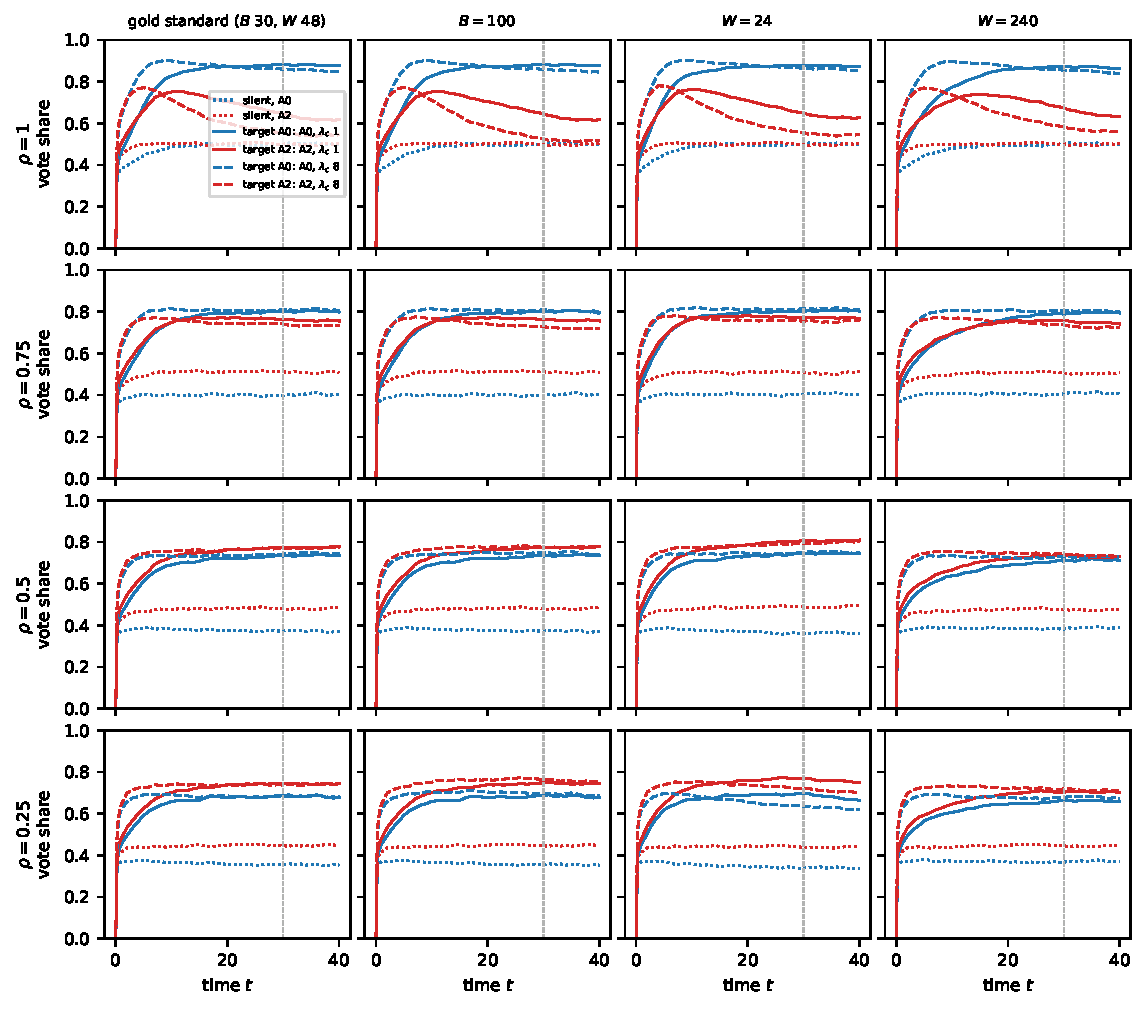
\includegraphics[width=0.98\linewidth]{figures/fig_votes.pdf}
\caption{Share of agents voting A0 (blue) and A2 (red), Eq.~(\ref{eq:share}): without a controller (dotted), with the
controller targeting A0 (blue) or A2 (red) at $\lambda_c = 1$ (solid) and $\lambda_c = 8$ (dashed). Rows: memory
$\rho$; columns: the four cases. $q = 6$, $q_c = 12$, gate on. At $t = 0$ nobody has voted and every share is 0.}
\label{fig:votes}
\end{figure}

\begin{itemize}\itemsep1pt
\item \textbf{Without a controller the swarm stays split in every case}: on $t = 30$ the A0 and A2 shares differ
  from the gold standard's by at most 0.02.
\item \textbf{Either controller still tips it at every memory, in every case.} The false controller's A2 share on
  $t = 30$ ($\lambda_c = 1$) is 0.77 (gold standard), 0.81 ($W = 24$) and 0.73 ($W = 240$) at $\rho = 0.5$; at $\rho = 1$
  it is 0.65, 0.65 and 0.67.
\item \textbf{The larger budget changes almost nothing}: at $\lambda_c = 8$, A2 on $t = 30$ goes from 0.77 to 0.78
  ($\rho = 0.5$) and from 0.55 to 0.53 ($\rho = 1$). In no case does the A2 share pass 0.81.
\item \textbf{The truth controller's A0 share stays within 0.03 of the gold standard} on $t = 30$, except $W = 24$ at
  $\rho = 0.25$, $\lambda_c = 8$ (0.63 against 0.68). Every result persists after the controller stops (from $t = 30$
  to 40 the shares change by at most 0.04).
\end{itemize}

\section{Observables as time series}\label{sec:time}

\begin{figure}[H]
\centering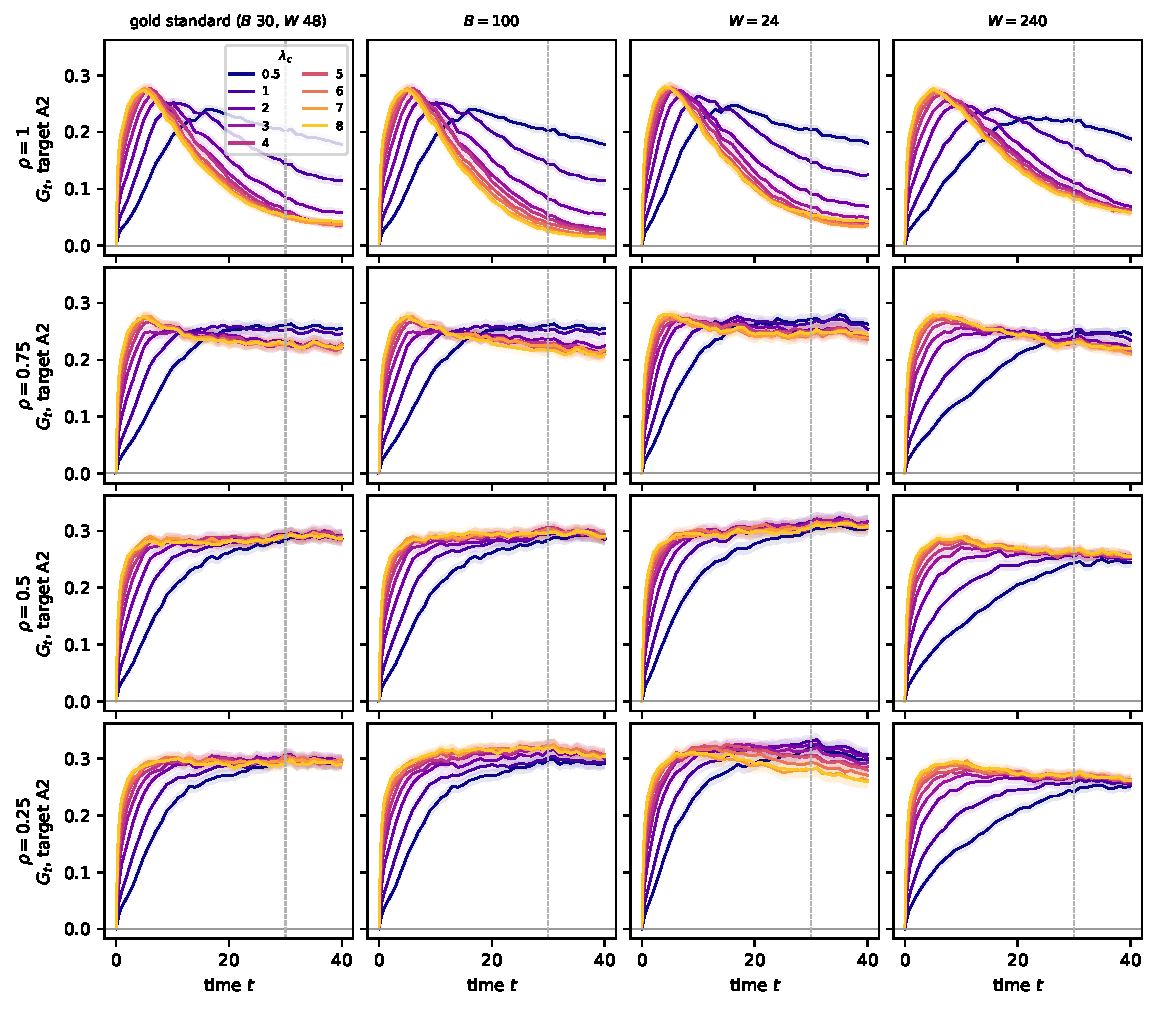
\includegraphics[width=0.98\linewidth]{figures/fig_gain_time_A2.pdf}
\caption{Paired susceptibility $G_t$ for target A2, Eq.~(\ref{eq:chi}), one curve per rate $\lambda_c$ (bands: 95\%
intervals); rows $\rho$, columns the four cases. $q = 6$, $q_c = 12$, gate on.}
\label{fig:gainA2}
\end{figure}

\begin{figure}[H]
\centering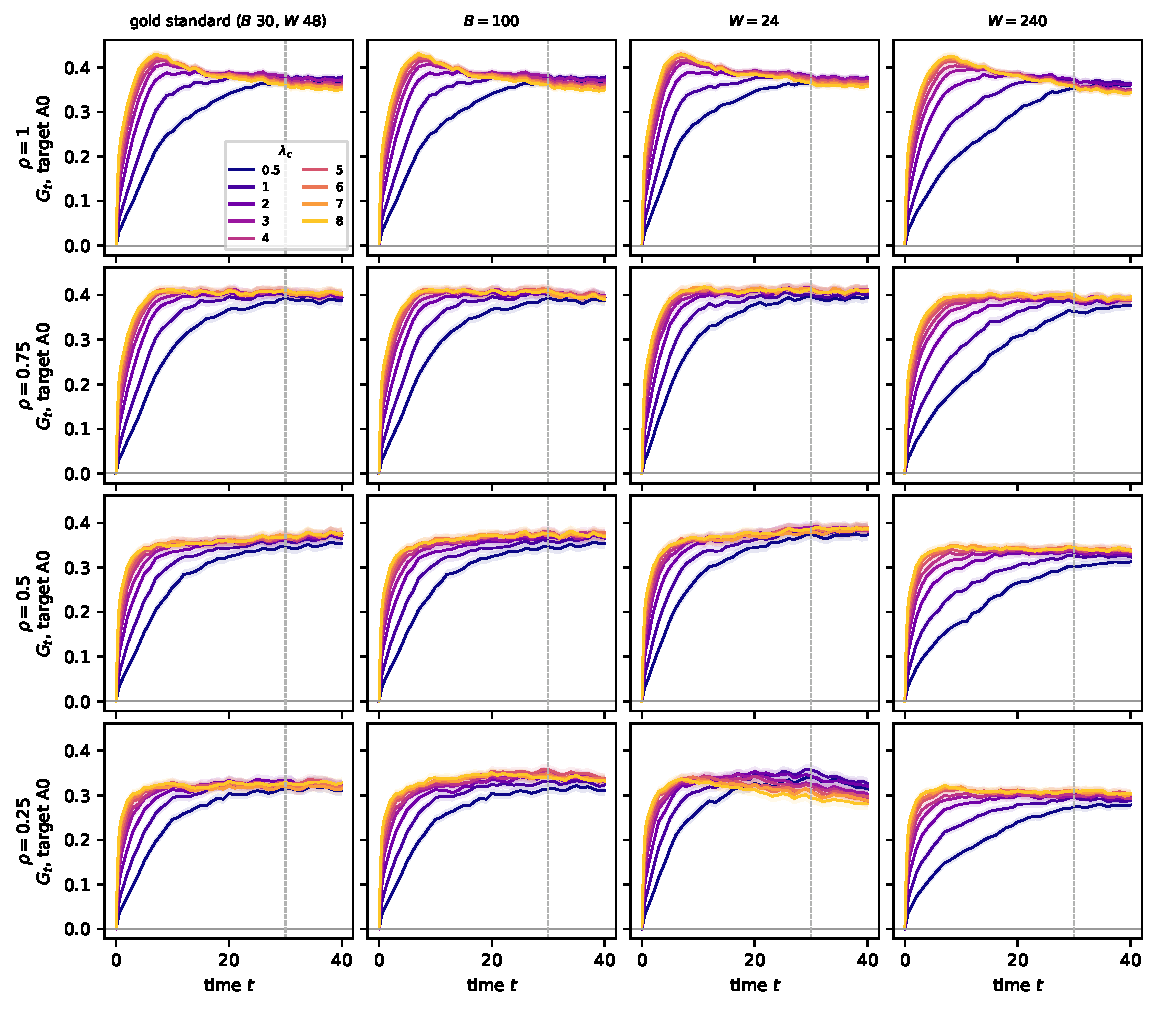
\includegraphics[width=0.98\linewidth]{figures/fig_gain_time_A0.pdf}
\caption{The same for target A0.}
\label{fig:gainA0}
\end{figure}

\paragraph{Susceptibility (Figures~\ref{fig:gainA2}, \ref{fig:gainA0}).}
\begin{itemize}\itemsep1pt
\item \textbf{$B = 100$ moves $G$ by at most 0.03}, for either target and every rate and memory, although the
  controllers post two to three times as many messages (false controller at $\lambda_c = 8$: 65--91 instead of 26--29).
\item \textbf{The window moves $G$ a little}: $W = 24$ by $-0.01$ to $+0.03$ (target A2); $W = 240$ by $-0.02$ to
  $-0.06$ at $\rho \le 0.5$ for target A2 and by up to $-0.05$ for target A0 at every memory.
\item \textbf{At full memory $W = 240$ helps the false controller} ($+0.02$ to $+0.04$), and the rate reversal of the
  gold standard weakens: $G$ falls from 0.22 ($\lambda_c = 0.5$) to 0.08 ($\lambda_c = 8$), against 0.20 to 0.05.
\end{itemize}

\begin{figure}[H]
\centering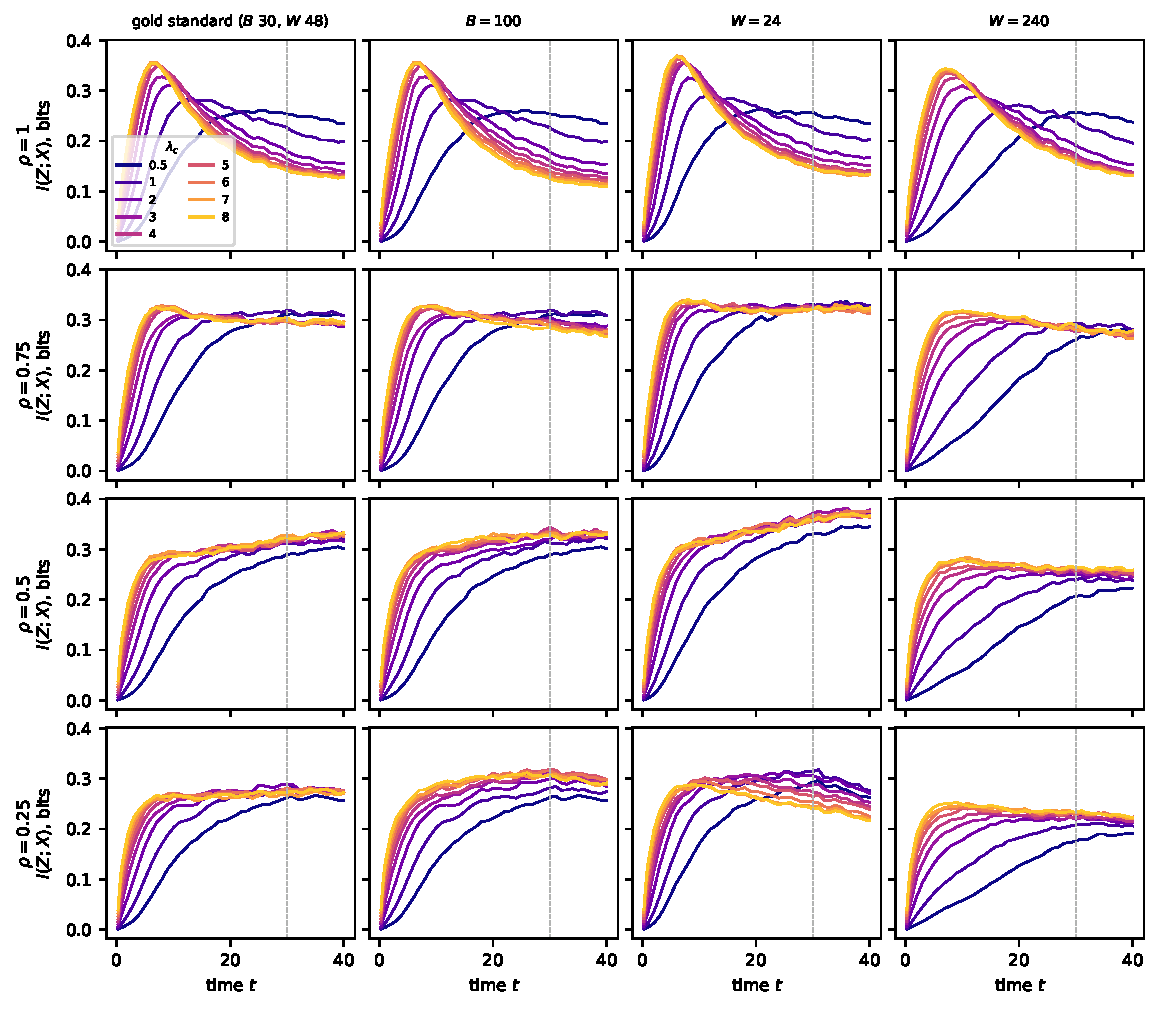
\includegraphics[width=0.98\linewidth]{figures/fig_info_time.pdf}
\caption{Readability $I(Z;X)$, Eq.~(\ref{eq:I}), one curve per rate; rows $\rho$, columns the four cases.}
\label{fig:info}
\end{figure}

\begin{figure}[H]
\centering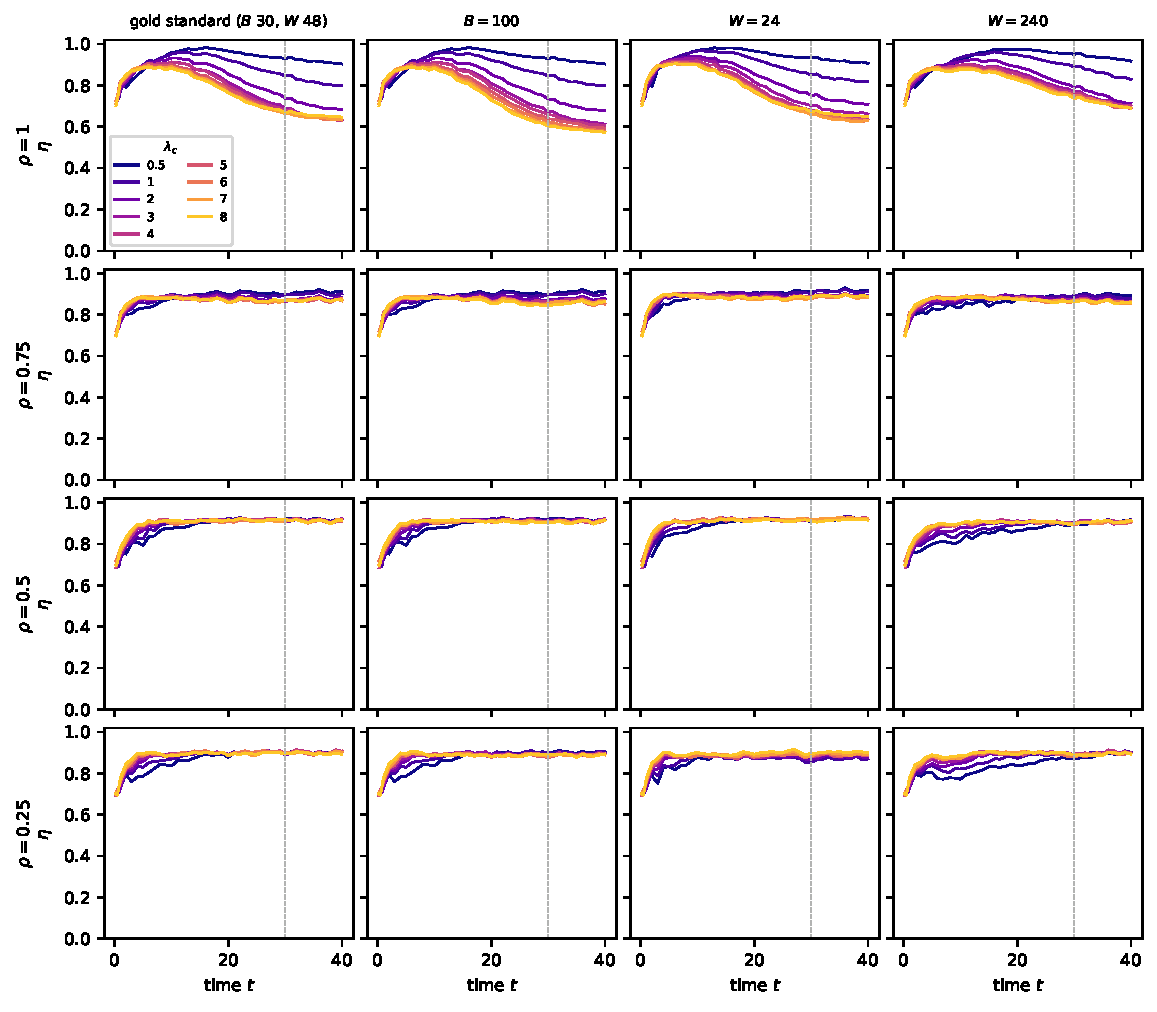
\includegraphics[width=0.98\linewidth]{figures/fig_eta_time.pdf}
\caption{Efficiency $\eta$, Eq.~(\ref{eq:eta}), one curve per rate (blank: undefined, $C < 0.01$ bits).}
\label{fig:eta}
\end{figure}

\paragraph{Readability and efficiency (Figures~\ref{fig:info}, \ref{fig:eta}).}
\begin{itemize}\itemsep1pt
\item \textbf{Readability follows the susceptibility}: on $t = 30$, $\rho = 0.5$, $I = 0.29$--$0.33$ bits (gold
  standard), $0.29$--$0.34$ ($B = 100$), $0.33$--$0.37$ ($W = 24$), $0.21$--$0.26$ ($W = 240$).
\item \textbf{The efficiency does not move}: $\eta = 0.84$--$0.92$ on $t = 30$ at $\rho < 1$ in every case; at
  $\rho = 1$ it spreads over the rates (0.60--0.95), as in the gold standard.
\end{itemize}

\begin{figure}[H]
\centering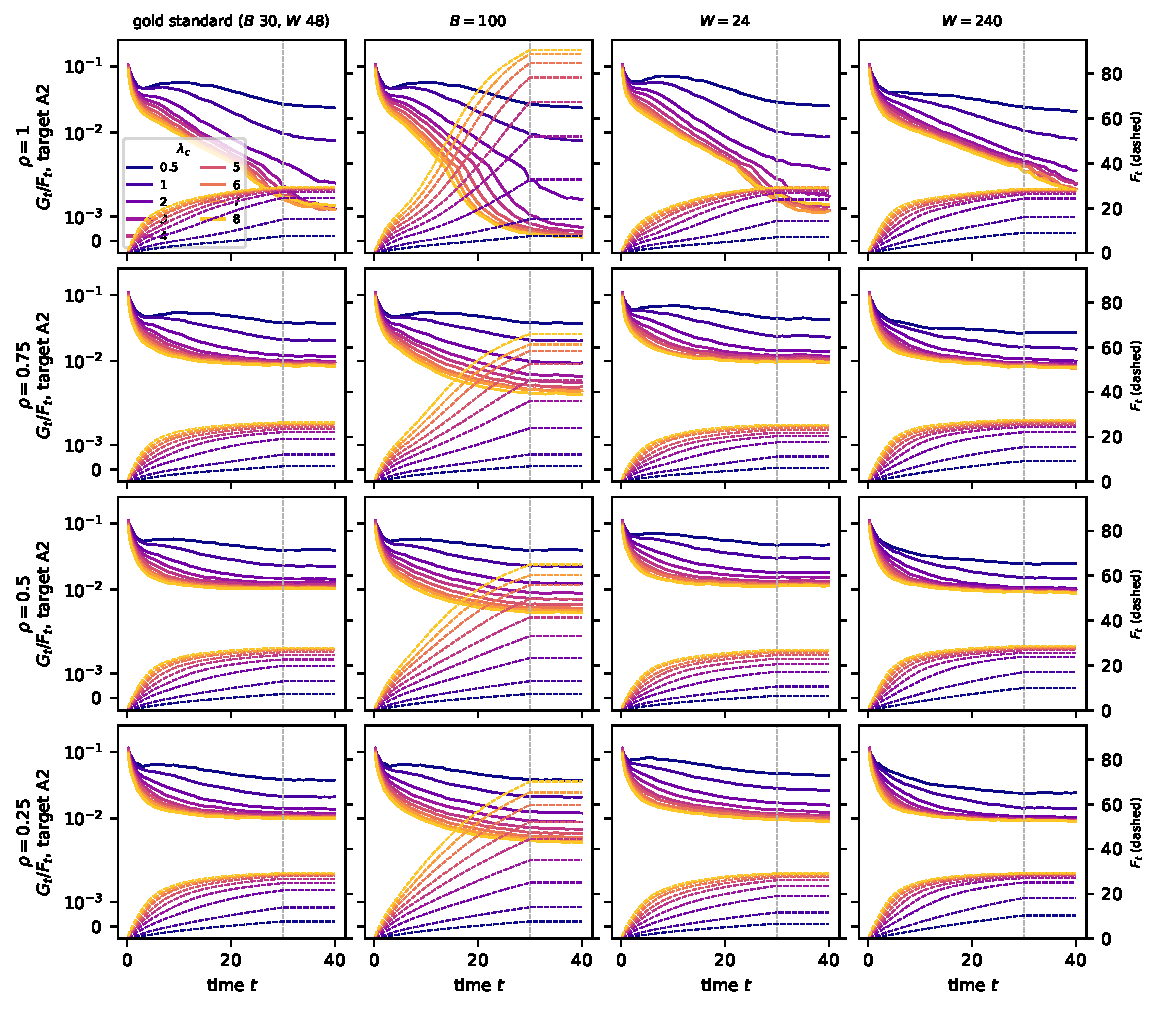
\includegraphics[width=0.98\linewidth]{figures/fig_per_fact.pdf}
\caption{Gain per message $G_t/F_t$ (solid, left axis, log scale; shown once half a message has been posted) and
messages posted $F_t$ (dashed, right axis), target A2, one colour per rate; rows $\rho$, columns the four cases.}
\label{fig:perfact}
\end{figure}

\paragraph{Gain per message (Figure~\ref{fig:perfact}).}
\begin{itemize}\itemsep1pt
\item \textbf{The extra messages of $B = 100$ are worth almost nothing}: on $t = 30$, $\lambda_c = 8$, the gain per
  message falls from 0.0104 to 0.0046 at $\rho = 0.5$ and from 0.0017 to 0.0003 at $\rho = 1$.
\item \textbf{The window changes the value of each message}: at $\lambda_c = 1$, $\rho = 0.5$: 0.030 ($W = 24$), 0.023
  (gold standard), 0.015 ($W = 240$).
\end{itemize}

\section{Phase diagrams}\label{sec:phase}

On $t = 30$, gate on; susceptibility for target A2 (grey number: its 95\% interval includes 0); readability and
efficiency for the pair of targets. The variants were run at $q_c = 12$ only, so the gold standard's
$q_c \times \lambda_c$ diagram has no counterpart.

\begin{figure}[H]
\centering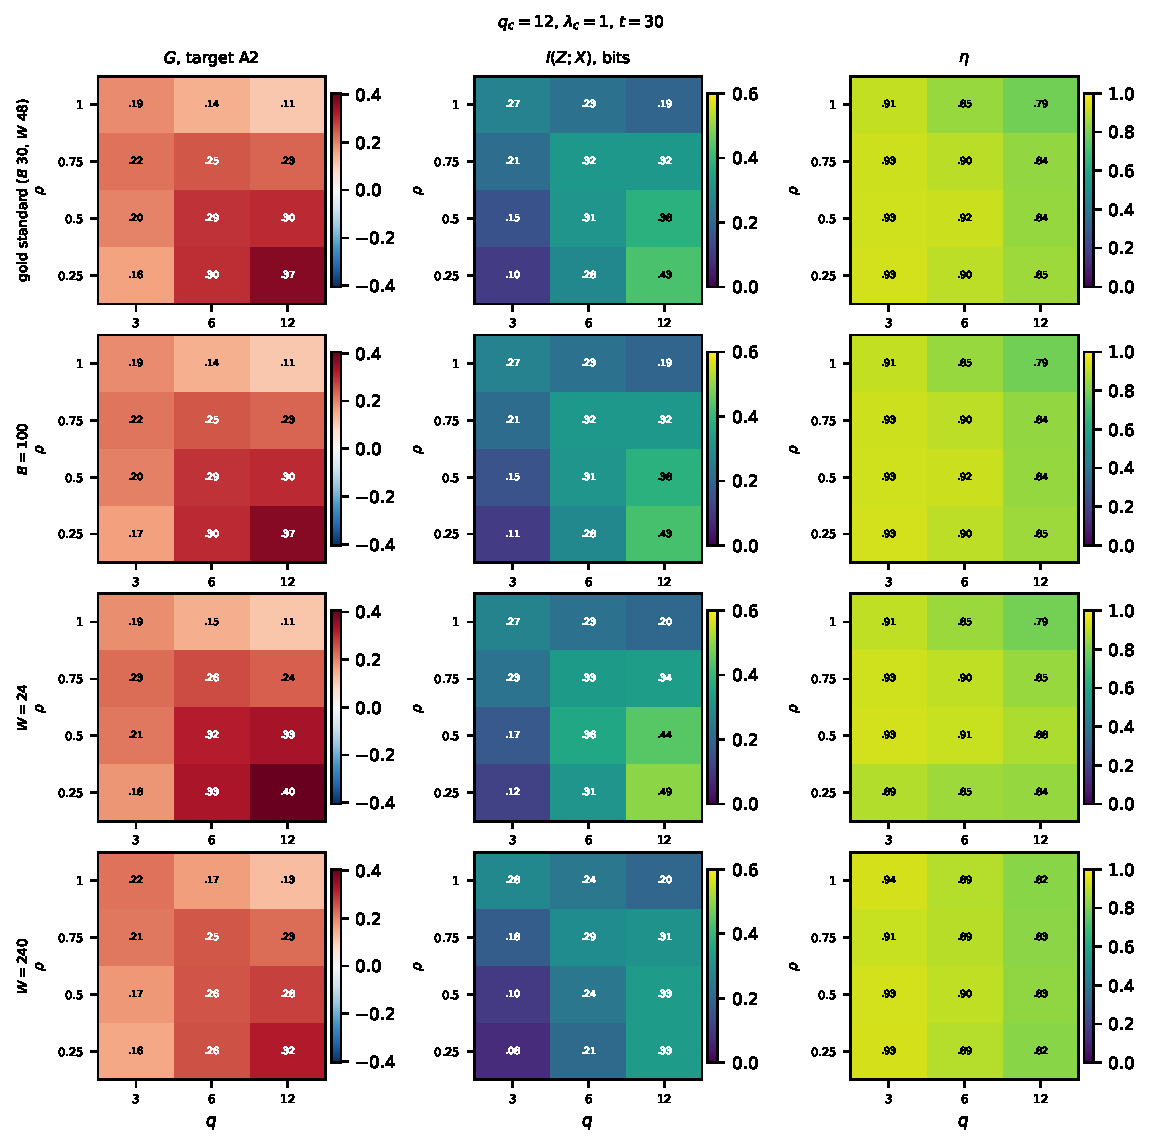
\includegraphics[width=0.92\linewidth]{figures/fig_phase_rho_q.pdf}
\caption{Susceptibility, readability and efficiency over memory $\rho$ and the posts each agent reads $q$; rows: the
four cases. $q_c = 12$, $\lambda_c = 1$.}
\label{fig:phaserq}
\end{figure}

\begin{itemize}\itemsep1pt
\item \textbf{The reading reversal survives in every case}: with full memory reading more hurts the controller ($G$
  from $q = 3$ to 12: 0.19 $\to$ 0.11 gold standard, $B = 100$ and $W = 24$; 0.22 $\to$ 0.13 $W = 240$); with heavy
  forgetting it helps (0.16 $\to$ 0.37 gold standard, 0.17 $\to$ 0.37 $B = 100$, 0.18 $\to$ 0.40 $W = 24$, 0.16 $\to$ 0.32 $W = 240$).
\end{itemize}

\begin{figure}[H]
\centering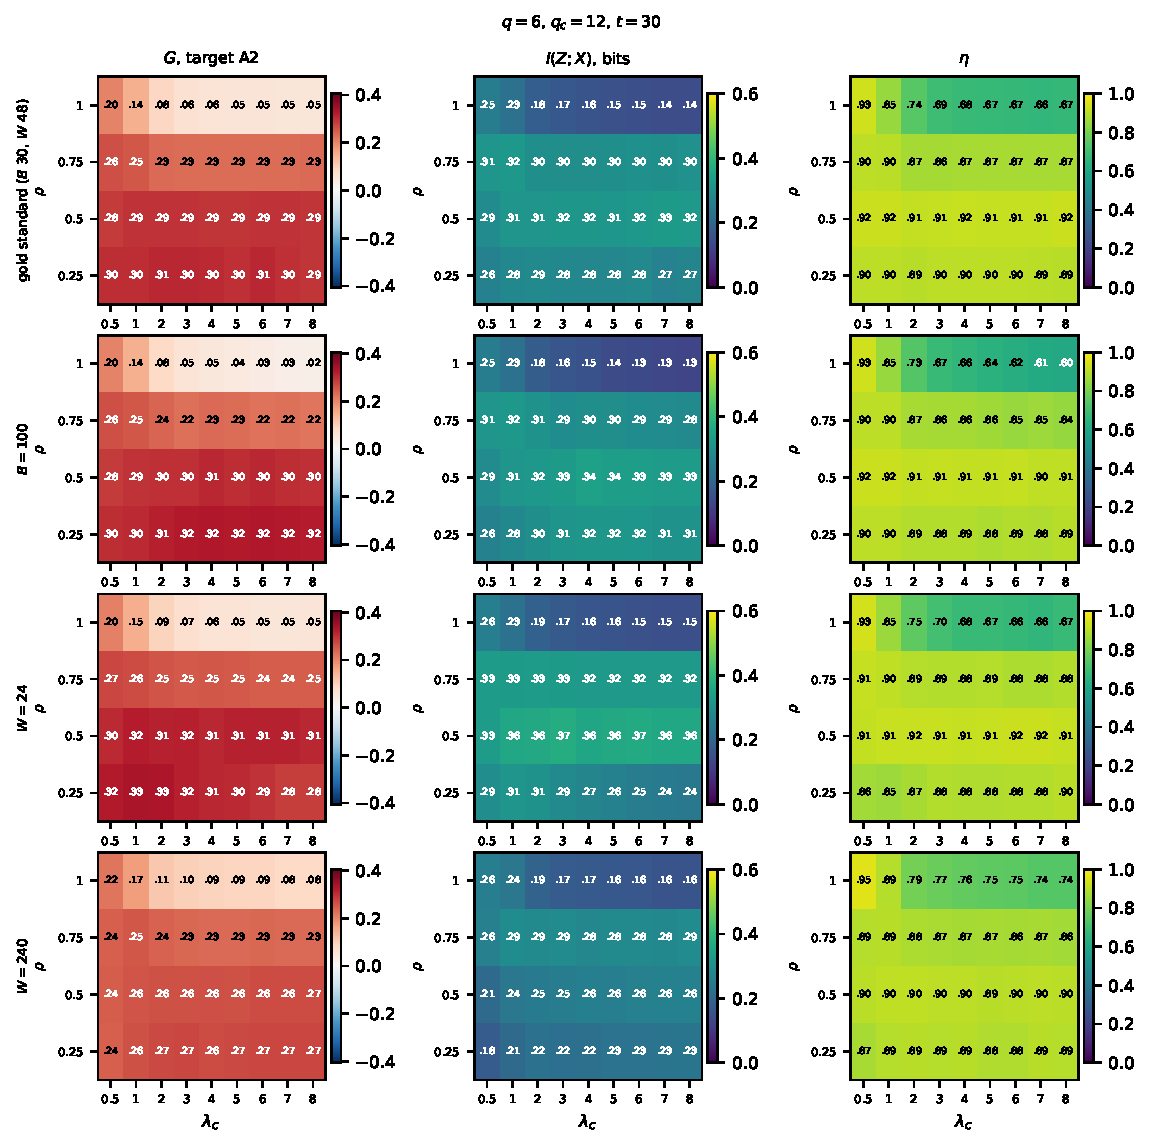
\includegraphics[width=0.92\linewidth]{figures/fig_phase_rho_x.pdf}
\caption{Susceptibility, readability and efficiency over memory $\rho$ and the rate $\lambda_c$; rows: the four
cases. $q = 6$, $q_c = 12$.}
\label{fig:phaserx}
\end{figure}

\begin{itemize}\itemsep1pt
\item \textbf{The rate hardly matters at $\rho < 1$ in any case}: from $\lambda_c = 1$ to 8, $G$ changes by at most
  0.05; at $\rho = 1$ it falls with the rate in every case.
\end{itemize}

\section{Susceptibility against the rate, against messages, and its slope}\label{sec:strength}

\begin{figure}[H]
\centering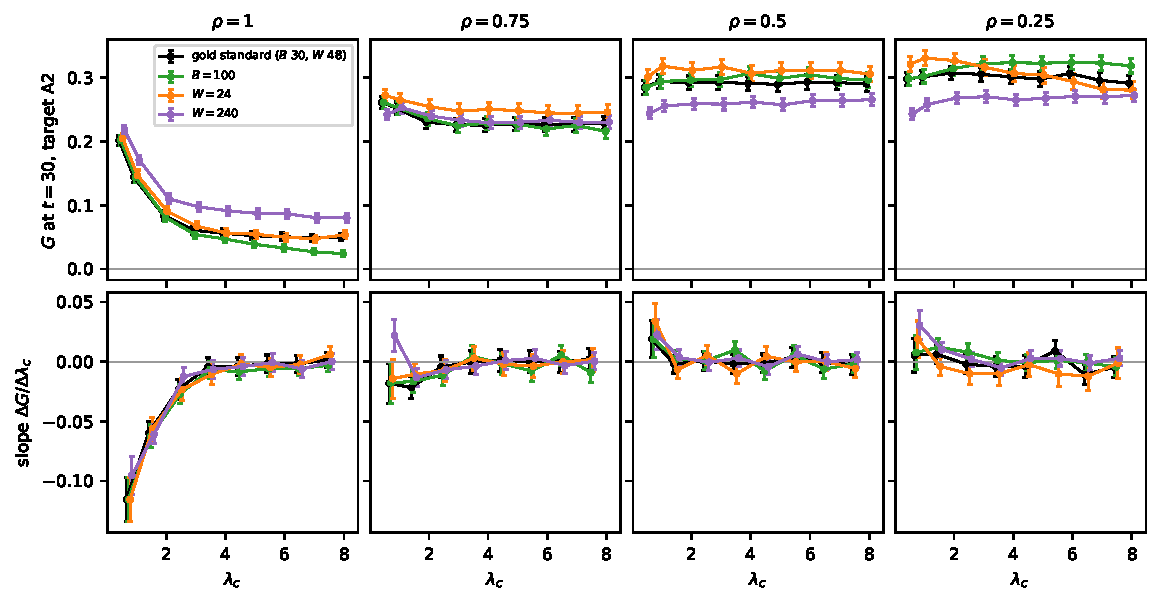
\includegraphics[width=0.98\linewidth]{figures/fig_gain_rate.pdf}
\caption{Top: $G$ on $t = 30$, target A2, against the rate $\lambda_c$, one colour per case (bars: 95\% intervals;
points shifted slightly sideways). Bottom: the slope between neighbouring rates, Eq.~(\ref{eq:slope}), with paired
95\% intervals. $q = 6$, $q_c = 12$, gate on.}
\label{fig:strength}
\end{figure}

\begin{figure}[H]
\centering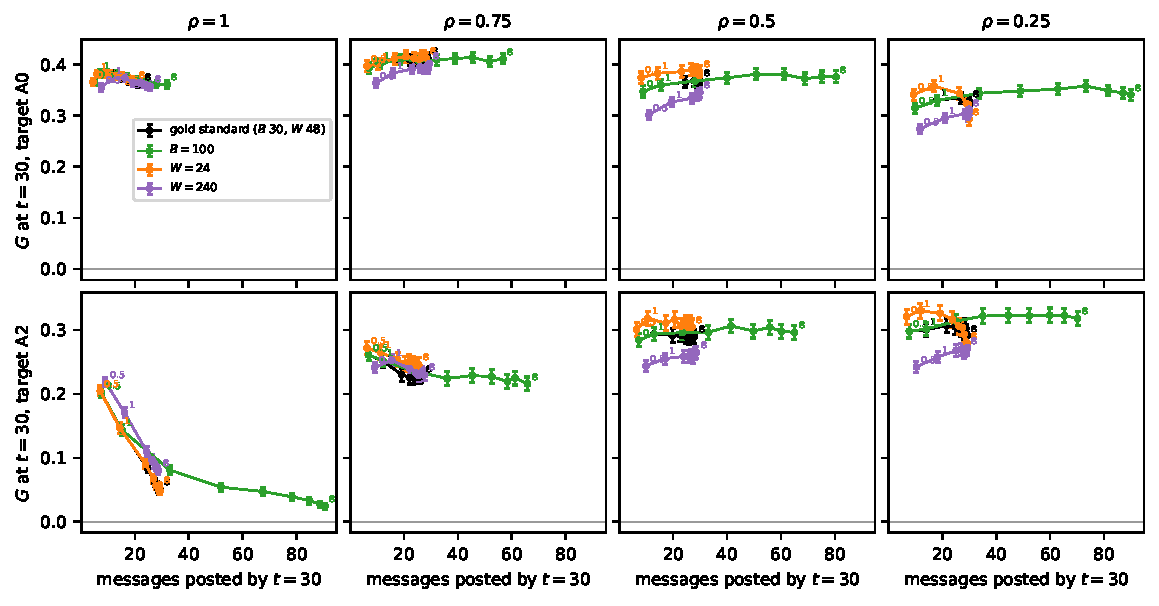
\includegraphics[width=0.98\linewidth]{figures/fig_gain_messages.pdf}
\caption{$G$ on $t = 30$ against the messages posted by then, one point per rate (labels: $\lambda_c$ = 0.5, 1, 8),
target A0 (top) and A2 (bottom), one colour per case; bars: 95\% intervals. Messages can repeat a fact: the pool
holds 12.}
\label{fig:messages}
\end{figure}

\begin{figure}[H]
\centering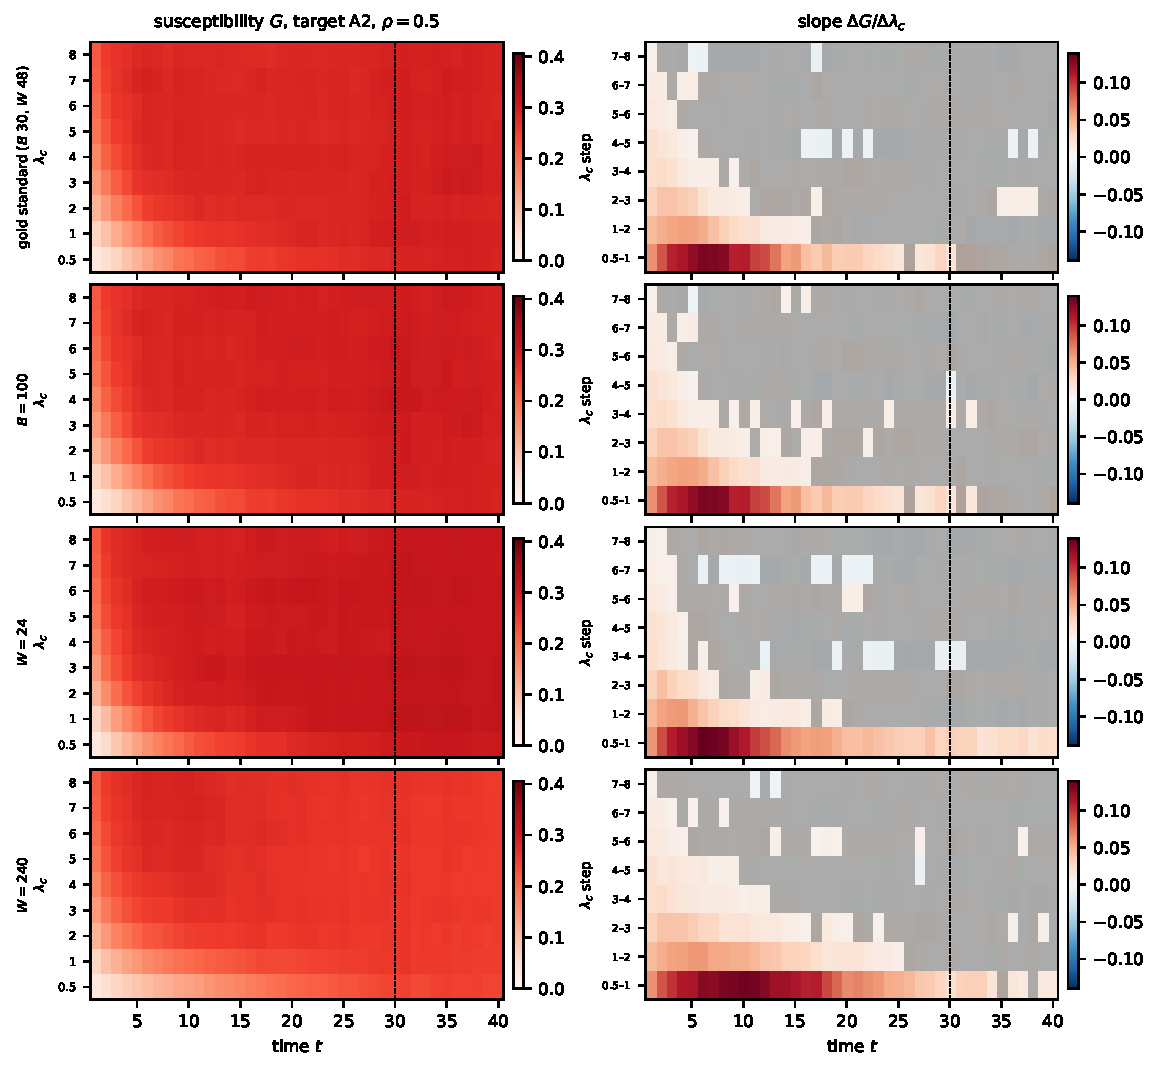
\includegraphics[width=0.92\linewidth]{figures/fig_strength_time.pdf}
\caption{$G$, target A2 (left), and its slope between neighbouring rates (right) over time ($x$) and rate ($y$),
$\rho = 0.5$; rows: the four cases. Faded cells: the paired 95\% interval of the slope includes 0.}
\label{fig:strengthtime}
\end{figure}

\begin{itemize}\itemsep1pt
\item \textbf{More messages do not raise the gain} (Figure~\ref{fig:messages}): with $B = 100$ the curves stretch to
  the right but stay flat; at $\rho = 0.5$ the false controller gains 0.28--0.31 whether it posts 13 or 65 messages.
\item \textbf{With full memory the rate reversal is there in every case}: the first step of rate costs $-0.12$ per
  unit (gold standard, $B = 100$, $W = 24$) or $-0.10$ ($W = 240$), the second $-0.06$ in every case. At $\rho < 1$ every
  significant slope is small ($|{\rm slope}| \le 0.034$).
\item \textbf{The gate matters little in every case}: gate off minus on, target A2, $t = 30$, is between $-0.08$ and
  $+0.03$, the largest effects at $\rho = 1$.
\end{itemize}

\paragraph{No proofs here.} In \texttt{task003-nosolution} no set of facts proves any allocation, so the
gold standard's ``who holds the proof'' section has no counterpart.

\section{Conclusions}

\begin{enumerate}\itemsep2pt
\item \textbf{The results of the 17 October nosolution report hold in all three variants}: either controller tips the
  swarm at every memory, full memory included; with full memory a faster controller gains less; reading more helps
  the controller when agents forget and hurts it when they remember; $\eta$ stays at 0.84--0.92 for $\rho < 1$.
\item \textbf{The budget does not matter here.} With $B = 100$ the controllers post two to three times as many
  messages and gain at most 0.03 more; the A2 share never passes 0.81. A likely reason, not tested: without a proof,
  an agent's belief is limited by what the facts imply, and once agents hold the controller's facts, repeating them
  adds nothing.
\item \textbf{The board's memory protects a little}: $W = 240$ lowers the false controller's gain by 0.02--0.06 at
  $\rho \le 0.5$ and the truth controller's by up to 0.05; $W = 24$ raises the false controller's by up to 0.03.
  At full memory $W = 240$ instead helps the false controller slightly and weakens the rate reversal.
\item \textbf{Compared with \texttt{task003-symmetric}}: there, a larger budget raised the false controller's gain by
  up to 0.13 and the window moved it by up to 0.14; here both effects are at most 0.06. Without a proof to erode,
  the swarm saturates after a few messages.
\end{enumerate}

\paragraph{Caveats.} The window changes what the controller reads too: with $W = 240$ its vote gate sees votes up to
10 time units old, and at $\lambda_c = 1$ it posts 15--18 messages instead of 12--15. The variants were run at
$q_c = 12$ and four memory values only. One world, 24 exact-Bayesian agents, one controller policy; 1{,}000 episodes
per setting (95\% intervals on $G$ about $\pm 0.02$). Data: \texttt{results/simulation\_2/2026-10-18\_sim2\_nosolution\_*};
tables: \texttt{results/gold\_standard/2026-10-18/} (variants) and \texttt{2026-10-16/} (gold standard); code:
\texttt{shared\_analysis/gold\_standard/make\_report\_figures\_2026-10-19.py}.

\end{document}
